\documentclass{sigchi}

\toappear{}

% Arabic page numbers for submission. 
% Remove this line to eliminate page numbers for the camera ready copy
\pagenumbering{arabic}


% Load basic packages
\usepackage{balance}  % to better equalize the last page
\usepackage{graphics} % for EPS, load graphicx instead
\usepackage{times}    % comment if you want LaTeX's default font
\usepackage{url}      % llt: nicely formatted URLs

\usepackage{tikz}
\usepackage{subfigure}
\usetikzlibrary{backgrounds,automata}

% llt: Define a global style for URLs, rather that the default one
\makeatletter
\def\url@leostyle{%
  \@ifundefined{selectfont}{\def\UrlFont{\sf}}{\def\UrlFont{\small\bf\ttfamily}}}
\makeatother
\urlstyle{leo}


% To make various LaTeX processors do the right thing with page size.
\def\pprw{8.5in}
\def\pprh{11in}
\special{papersize=\pprw,\pprh}
\setlength{\paperwidth}{\pprw}
\setlength{\paperheight}{\pprh}
\setlength{\pdfpagewidth}{\pprw}
\setlength{\pdfpageheight}{\pprh}

%====================%
%====================%

\newcommand{\cs}{C\slash S}
\usepackage {mdwlist}
%====================%
%====================%


% Make sure hyperref comes last of your loaded packages, 
% to give it a fighting chance of not being over-written, 
% since its job is to redefine many LaTeX commands.
\usepackage[pdftex]{hyperref}
\hypersetup{
pdftitle={SIGCHI Conference Proceedings Format},
pdfauthor={LaTeX},
pdfkeywords={SIGCHI, proceedings, archival format},
bookmarksnumbered,
pdfstartview={FitH},
colorlinks,
citecolor=black,
filecolor=black,
linkcolor=black,
urlcolor=black,
breaklinks=true,
}

% create a shortcut to typeset table headings
\newcommand\tabhead[1]{\small\textbf{#1}}


% End of preamble. Here it comes the document.


\begin{document}

\title{Egal: Making Peer-to-Peer Games over Named Data Network}

\numberofauthors{3}
\author{
  \alignauthor 1st Author Name\\
    \affaddr{Affiliation}\\
    \affaddr{Address}\\
    \email{e-mail address}\\
%    \affaddr{Optional phone number}
  \alignauthor 2nd Author Name\\
    \affaddr{Affiliation}\\
    \affaddr{Address}\\
    \email{e-mail address}\\
%    \affaddr{Optional phone number}    
  \alignauthor 3rd Author Name\\
    \affaddr{Affiliation}\\
    \affaddr{Address}\\
    \email{e-mail address}\\
%    \affaddr{Optional phone number}
}

% Teaser figure can go here
% \teaser{
%  \centering
%  \includegraphics{Figure1}
%  \caption{Teaser Image}
%  \label{fig:teaser}
%}

\maketitle

%====================%
%====================%
\begin{abstract}
%
\end{abstract}

\keywords{}



%====================%
%====================%

\section{Introduction}
\label{introduction}
% (*gamer / player / customer / peer)    (publisher / carrier / *operator / service provider)
% "the" is really the most difficult word in English! on "the" one hand ...
% I mentioned security and cheating avoidance here. I'd better include them in Discussions
% I set the importance order: consistency, scalability, security. I'd better follow this order

% Requirements of Networked Games %
Requirements of massive multiplayer online games (MMOG) from both operators and gamers have been rising. On the one hand, gamers like games that are \emph{interactive}: games should be responsive to user input, and ideally should provide multiple channels for inter-person communication. On the other hand, gamers equally care about \emph{consistency}: all participants should have an equal understanding of the game state at any time, unless it is decided by the game rules. Few customers would be glad if they were told that \emph{interactivity} and \emph{consistency} are two contradicting requirements, though it is indeed the case. To make things worse, requirements from operators are no less complex than those from gamers. First, they want the game system to be \emph{scalable}: service quality should not fall dramatically when the number of gamers is large or is rapidly growing. Second, bandwidth consumption should be minimized for financial reasons. Third, just like any service providers they want a \emph{security} model to survive from attacks. Finally, game operators specially want to \emph{avoid cheating} on behalf of honest gamers.

% NDN Features %
In~\cite{Jndn}~the authors proposed \emph{Contnet-Centric Network} (CCN) or \emph{Named Data Network} (NDN), a second generation Internet architecture that reduces network traffic and achieves scalability, security and performance simultaneously (see section \nameref{ndnbg}). NDN treats content as a primitive in stead of location, and retrieves a content by its name instead of its IP address. By making use of web cache, NDN improves content distribution efficiency and reduces traffic. Its one-for-one flow control gives the network scalability and adaptability. Security is embodied in content, which is more trustworthy than securing connections and hosts.

% Motivations of the Paper %
Because NDN has these appealing features, we would like to explore its capability of solving game-related problems. We developed the Egal library which is a C\# wrapper of native NDN code and would allow for fast prototyping. Using the library, we adapted an open source car racing game into a peer-to-peer NDN game. Meanwhile, we studied the requirements of consistency, scalability and security in the context of NDN. Our experience would work as an example for future NDN game designers and our library could be reused by future developers.

% About Following Sections %
% not so sure %
We include concepts from both game design and NDN in section \nameref{background}. In section \nameref{gamedesign} we present our sample game and its consistency maintenance mechanism. Section \nameref{implementation} reveals the general approach to developing games on NDN. Then in section \nameref{discussions} we compare NDN games with traditional ones on bandwidth requirement, security and cheating avoidance.




%====================%
%====================%
\section{BACKGROUND}
\label{background}

% not so sure %
% In this section we put game design and NDN side by side and summarize concepts, from both realm, that are most closely related to consistency, scalability and security.

%-----------------------------------%
\subsection{Game Design Background}
\label{gamedesignbg}

% (scalability -- architecture)  (consistency -- synchronization algorithm) %
The scalability of a system is closely related to its architecture. In an unscalable architecture, when the client number increases resource bottlenecks would appear, reducing system overall performance. Depending on which architecture is used, a system may need a synchronization mechanism to maintain consistency. Security and cheating avoidance strategies are also architecture-dependent.

% . . . . . . . . . . . . . . . . . . . . . . . %
\subsubsection{Game Architectures}
\label{game_archi}

% C/S and P2P %
Game architecture are usually classified as Client\slash Server (\cs) or peer-to-peer (P2P). 

In {\cs} architectures (figure~\ref{cs}) all clients are connected to a central server which receives client events, authenticate, compute and publish updates of global game state. The only two responsibilities of clients are sending user input to the server and rendering the new game state received from it. This centralized model intrinsically guarantees consistency, as there is only one source of global game state. However, the server is also the resource bottleneck, rendering the system unscalable. This architecture is not robust as the server is a single point of failure. Finally the server introduces additional latency.

In contrast, in P2P architectures (figure~\ref{p2p}) there is no central authority. Clients, or peers are interconnected with each other and each peer maintains its own copy of the game state. Player authentication and game state computation are decentralized and peers send messages asynchronously to inform updates. Because P2P architectures resource-growing~\cite{Scheating}, they are scalable. Because peers send messages directly to each other, network latency is minimized. However, P2P architectures require synchronization mechanisms to guarantee the consistency of the replicated game state among peers. Cheating is also easier in P2P than it is in {\cs}.

\begin{figure} 
\centering  
\subfigure[\cs]  
{  
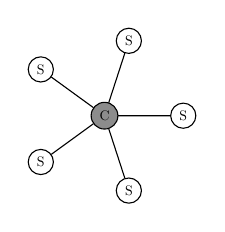
\begin{tikzpicture} [scale=0.5, transform shape]
\tikzstyle{every node}=[draw,shape=circle];
\node [fill = gray!90] (v0) at (0:0) {C};
\node (v1) at ( 0:2) {S};
\node (v2) at ( 72:2) {S};
\node (v3) at (2*72:2) {S};
\node (v4) at (3*72:2) {S};
\node (v5) at (4*72:2) {S};
\draw (v0) -- (v1) % star
(v0) -- (v2)
(v0) -- (v3)
(v0) -- (v4)
(v0) -- (v5);
\end{tikzpicture}
\label{cs}
}  
\subfigure[P2P]  
{  
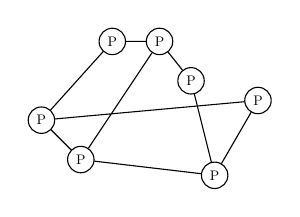
\begin{tikzpicture} [scale=0.5, transform shape]
\tikzstyle{every node}=[draw,shape=circle];
\node (v0) at (0, 2) {P};
\node (v1) at (1, 1) {P};
\node (v2) at (1.8, 4) {P};
\node (v3) at (3, 4) {P};
\node (v4) at (4.4, 0.6) {P};
\node (v5) at (3.8, 3) {P};
\node (v6) at (5.5, 2.5) {P};
\draw (v0) -- (v1)
(v0) -- (v2)
(v0) -- (v6)
(v4) -- (v5)
(v1) -- (v4)
(v2) -- (v3)
(v3) -- (v5)
(v4) -- (v6)
(v3) -- (v1);
\end{tikzpicture}
\label{p2p}
}
\caption{\cs~and P2P architectures}
\end{figure}

Hybrids of {\cs} and P2P exist: Mirrored Game Servers, Distributed Scene Graphs and many more. These architectures are described in~\cite{Ldsg, Scheating, Fgame, Csync}.


% . . . . . . . . . . . . . . . . . . . . . . . %
\subsubsection{Synchronization Mechanisms}
\label{syncalgr}

% conservative and optimistic %
The simplest way to maintain consistency among peers is to use totally ordered service, which is often not available. Therefore conservative and optimistic synchronization algorithms have been proposed to prevent or detect (and then correct) misorderings~\cite{Fgame}. 

Conservative synchronization algorithms would allow each peer to process received events only if it is safe to process them. Newly arrived events are usually delayed for an amount of time and the synchronization algorithm can determine the correct execution order. Famous examples are \emph{Chandy-Misra-Bryant algorithm}~\cite{Chandy, Bryant}, \emph{Lockstep synchronization}~\cite{Flockstep} and \emph{fixed time-bucket synchronization}. % Conservative algorithms do not exploit concurrency well and the delay they introduce will reduce interactivity.

Optimistic synchronization algorithms assume received events are in correct order and process them without delay. Then, if late events arrived a \emph{rollback} will be performed and all those optimistically executed events should be canceled and reprocessed. In order to rollback, large memory will used to take multiple snapshots of game state. Also, a mechanism to determine the early bound of rollback (for example the \emph{Global Virtual Time}) will be mandatory. The most famous optimistic synchronization algorithms are: \emph{Time Warp}, \emph{trailing state synchronization}~\cite{Csync}~and \emph{optimistic time-bucket synchronization}~\cite{Doptbkt}.

%-----------------------------------%
\subsection{NDN Background}
\label{ndnbg}

% Basic Exchange %
NDN \emph{names} can be human-readable (for example \url{/Egal/Car/Scene0}). Their binary encodings can be used for routing using longest prefix match.

NDN is designed for content distribution. Two packet types exists in NDN: \emph{Interest} and \emph{Data} (see figure~\ref{packet_types}). A data receiver first initiates an Interest packet that bears the \emph{name} of the \emph{content} it wants. The packet is then routed by name until it reaches a host that has the corresponding content. The matching content object is sent back as a Data packet, satisfying all Interest for it on its way and leaving a trail of `bread crumbs'~\cite{Jndn}~in the routers' memory. Later Interests for the same content may be directly satisfied by the routers. It is guaranteed that in NDN every piece of data would flow through a link for at most once. This would reduce a huge amount of network traffic around content distribution centers.

\begin{figure} 
\begin{center}
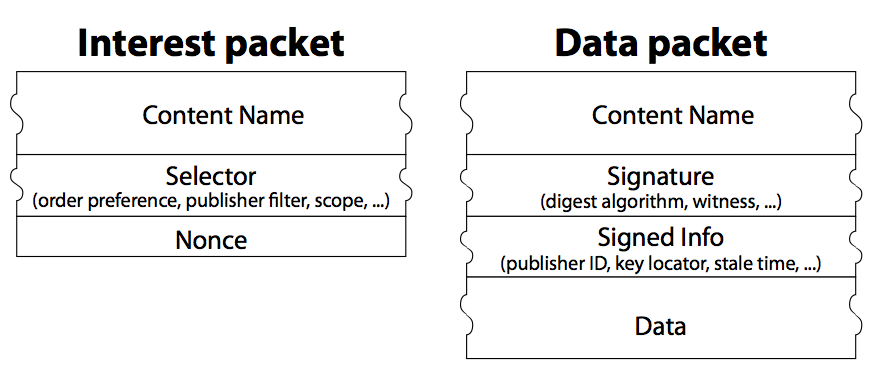
\includegraphics[width=0.4\textwidth] {image/packet_types}
\caption{packet types in NDN}
\label{packet_types}
\end{center}
\end{figure}

Note that NDN is receiver driven. Flow balance is also controlled by the receiver~\cite{Zact}. Also note that multicasting is intrinsically built in.

% . . . . . . . . . . . . . . . . . . . . . . . %
\subsubsection{CCNx Sync Protocol}
\label{ccnsync}

The CCNx Sync protocol allows applications to define collections of named data in \emph{repositories} that are to be automatically kept in sync with identically defined collections in neighboring repositories~\cite{CCNxSync}. A collection in the repository is also called a \emph{slice}. A local \emph{Sync Agent} builds and manages a \emph{Sync Tree} for a slice, using names that represent the content of the slice. Hashes of Sync Trees are sent among neighboring Sync Agents to detect any discrepancy. Once detected, normal Interest and Data packets will be sent for inconsistent data.

CCNx Sync protocol should not be confused with the game synchronization protocols mentioned in~\nameref{syncalgr}. CCNx Sync maintains data integrity: it keeps local repository slices coherent remote ones. Game synchronization algorithms provide a higher level service: they ensure that sync actions will be taken \emph{in order}.



%====================%
%====================%
\section{NDN GAME DESIGN}
\label{gamedesign}


% intro %
% not so sure %
In this section we present game design issues that are specific to NDN games. In most places we use our game adapted from the Unity3D Car Tutorial~\cite{UnityCar} as examples but we are not restricted to this genre.


%-----------------------------------%
\subsection{P2P Game Architecture}

% why did we choose P2P %
We decided that our sample game should be P2P because of the following reasons. First, P2P architectures are scalable and robust, with minimized network latency (see \nameref{game_archi}). Second, these advantages of P2P can be further enhanced by NDN. NDN reduces traffic in the network, which means that given the same bandwidth, more players could join the game. With data packets cached in the network, data receivers will enjoy a even smaller latency. Third, some of the disadvantages of P2P can be (partly) overcame by NDN. Security, for example, will be enhanced by NDN's content validation and trust management scheme. By naming contents instead of hosts, it will be more difficult for attackers to focus on their target. Several types of cheating behavior can be automatically avoided by NDN (see \nameref{discussions}). Finally, improvements on P2P architectures will also benefit the hybrid architectures. As an example, the Mirrored Game Server architecture has its clients connected to a local server, but typically orchestrates its distributed servers into a high-performance P2P network, so NDN could positively affect it in a similar way.


%-----------------------------------%
\subsection{Namespace Design}

% what is a namespace %
Namespace designing is a task specific to NDN application developers. A complete \emph{namespace} of a program is a full collection of names that will be used during the program's execution. Namespace can be presented as trees. For instance, figure~\ref{namespace} is the namespace of our sample car racing game. It is composed of three trees: a \emph{repo tree}, a \emph{network tree} and \emph{game tree}. Each tree node is contains one or more NDN name component(s). One can learn the major functionalities of an application by looking at its namespace design.

\begin{figure}
\begin{center}
\begin{subfigure} [Repo Tree]
{
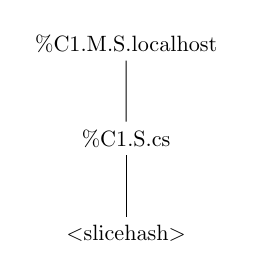
\begin{tikzpicture} [scale=0.8, transform shape]
    %\tikzstyle{every node}=[rectangle,draw]
    \node {\%C1.M.S.localhost}
        child { node {\%C1.S.cs} 
        		child{ node {$<$slicehash$>$} }
        }
       
    ;
\end{tikzpicture}
\label{repo}
}
\end{subfigure}
\begin{subfigure} [Network Tree]
{
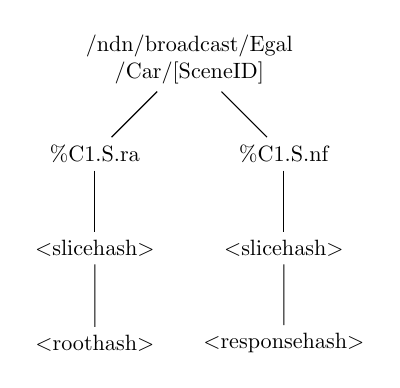
\begin{tikzpicture} [scale=0.8, transform shape]
    \tikzstyle{every node}=[align = center]
    \tikzstyle{level 1} = [sibling distance=30mm]
    \node {/ndn/broadcast/Egal \\ /Car/[SceneID]}
        child { node {\%C1.S.ra} 
        		child { node {$<$slicehash$>$} 
			child { node {$<$roothash$>$} }
		}
        }
        child { node {\%C1.S.nf}
        		child { node {$<$slicehash$>$} 
			child { node {$<$responsehash$>$} }
		}
        }
    ;
\end{tikzpicture}
\label{broadcast}
}
\end{subfigure}
\begin{subfigure} [Game Tree]
{
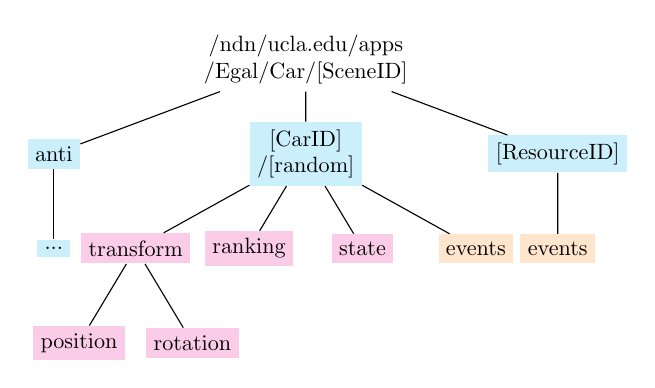
\begin{tikzpicture} [scale=0.8, transform shape]
    \tikzstyle{every node} = [align=center]
    \tikzstyle{asset} = [fill=cyan!20]
    \tikzstyle{state} = [fill=magenta!20]
    \tikzstyle{event} = [fill=orange!20]
    \tikzstyle{level 1} = [sibling distance=40mm]
    \tikzstyle{level 2} = [sibling distance=18mm]
    \node {/ndn/ucla.edu/apps \\ /Egal/Car/[SceneID]}
        child{ node [asset] {anti}
        		child { node [asset] {...}}
        }
        child { node [asset] { [CarID] \\ /[random]} 
		child { node [state] {transform} 
			child{ node [state] {position} }
			child{ node [state] {rotation} }
		}
		child { node [state] {ranking} }
		child { node [state] {state} }
		child { node [event] {events} }
        } 
         child { node [asset] {[ResourceID]}
        		child {node [event] {events}} }
        
    ;
\end{tikzpicture}
\label{game}
}
\end{subfigure}
\caption[Caption for LOF]{Namespace of our sample car racing game\footnotemark}
\label{namespace}
\end{center}
\end{figure}
\footnotetext{Colors of the nodes will be explained in \nameref{ase}. Nodes surrounded by $< >$ will be generated at run time using algorithms chosen by NDN. Nodes surrounded by $[ ]$ are variables that will be substituted with multiple values. Note that \slash~are not part of NDN names, they are for illustration purpose only.}


% localhost namespace: repo %
Names in the Repo Tree are used for communication with the local repository: we use CCNx Create Collection Protocol to create a slice, which is a collection of content objects with a common name prefix. Two parameters are used to define the slice: \emph{topo} and \emph{prefix}. They later become the root node of the network tree and the game tree. \url{\%C1.M.S.localhost} restricts the scope to the local node; \url{\%C1.S.cs} is a command marker for the Create Slice Interest~\cite{CCNxCS}. 

% SYNC namespace: [SceneID] %
The network tree illustrates names used by the CCNx Sync Protocol. This protocol is used for name discovery, which explains why its Interests are broadcasted on the NDN testbed (see its root node \url{/ndn/broadcast/...}). Note the use of \url{[SceneID]} in the namespace, which indicates that each scene will have its own slice and be synchronized independently. For small game this may not be necessary; for large games this might be replaced with \url{[DistrictID]} or \url{[BlockID]}. \url{\%C1.S.ra} and \url{\%C1.S.nf} are command markers for the Root Advice Interest and the Node Fetch Interest respectively~\cite{CCNxSync}.

% <nonce> says a lot %
The game tree is most closely related to the object hierarchy in the virtual world. In fact, a big portion of the tree is constructed by extracting objects and their member variables that needs to be transmitted through network. Please note the use of \url{[random]} in the namespace. In a car racing game each car should have a unique identifier in the network, therefore we append a \url{[random]} after \url{[CarID]} to reduce the probability of name collision. \url{[random]} can be omitted only if it is guaranteed by the application that  \url{[CarID]}  would not collide with one another. The same applies to most user-controlled avatars (first person shooters, heroes played by gamers etc.). However, with global virtual resources (such as a potion, a weapon or a bomb) and program controlled avatars (for example a bot enemy), the opposite is the case. The \url{[ResourceID]} in the namespace should never be combined with \url{[random]} and should be named systematically by the application. Otherwise illegal duplications of the resource would plague in the virtual world. 

% namespace for transmission optimization %
The game tree is designed for optimal transmission and does not have to resemble to the game's object hierarchy. In fact, names for immutable objects and static variables almost never appear in the game tree. The reason for excluding immutable objects is quite obvious: they should be \emph{installed} with the software, not \emph{transmitted} through the network. The exclusion of the terrain object in our game tree is a case in point. As for static variables, they should be \emph{initialized} with their parent object (if there is one) and thus can be omitted in many cases. An example for this is our \url{[ResourceID]} node. A resource object in our game has many static members (position, value etc.), which are initialized when the resource is dynamically created. Based on this observation, during synchronization we can pack these constant member variables as a content object and name it after the resource's name. The result is that none of these members become a child node of \url{[ResourceID]} in the game tree. On the other hand, names with little meaning in the virtual world might be added to the game tree just for transmission convenience. The node \url{state}, for example, is not a member variable of the \url{car} class, but a \emph{summary} of all variables under \url{[CarID]/[random]}. 
%In other words, if $transform = \{  \{ x_p, y_p, z_p, t_0\},  \{ x_r, y_r, z_r, t_1\}  \}$ and $ranking = \{  r, t_2\}$, then $state = \{ x_p, y_p, z_p, x_r, y_r, z_r, r, max(t_0, t_1, t_2) \}$. 
Hence, for a peer who is interested in \url{Car0}'s updates, issuing an Interest for the \url{state} is more efficient than sending three packets for \url{position}, \url{rotation} and \url{ranking}.
\footnote{Note that the peer cannot just issue an Interest for \url{car0} and hope to get all the content. An Interest like that will be replied with \url{car0} or one of its children and the peer would not know which child it is until the data packet is received.}

Such name components as \url{state} can have many variations that serve different purposes. For example, an object may want to keep two summaries of different detail levels: a \url{short} summary and a \url{long} summary. The longer summary might interest players who are directly interacting with the object while the shorter one can be used by distant players for the integrity of their global view. Name components can also be \url{public} (for everyone including enemies) or \url{private} (and encrypted, for group members only). An \url{invisible} name component can be used to provide a summary that does not have position information. In effect, this hides a player from others' view. The interesting fact that name components are not restricted to nouns may inspire NDN developers to design namespaces that are rich in meaning and functionalities.



%====================%
%====================%
\section{Synchronization}
\label{sync}

The purpose of synchronization is to maintain consistent views of the global game state for all players. The definition of global game state varies from author to author, but it generally means the combined state of all entities (players, non-player characters and objects) in the game. In NDN in particular, the global game state is equivalent to the game tree (figure~\ref{game}) and all its corresponding content objects. Hence, to synchronize a NDN multiplayer on-line game is to synchronize its game tree and all the content objects that underlies.

We divide the problem of synchronizing the game tree into three sub-problems: Asset synchronization, State synchronization and Event synchronization. We recognize nodes in the game tree as \emph{asset}s, \emph{state} and \emph{event}s and use choose different strategies to synchronize them. The idea behind such a division is that assets, state and events have different requirements for synchronization.

%-----------------------------------%
\subsection{Asset, State and Event}
\label{ase}

Asset, state and event are the three classes of content that need to be synchronized. In figure~\ref{game} for example, all asset names are colored blue, all state nodes pink and all event nodes yellow. A formal definition is as follows:
\begin{description*} 
\item [Asset]
A node in the game tree whose presence and absence \emph{cannot} be deduced from the presence and absence of its parent node.
\item [State]
A node in the game tree whose presence and absence \emph{can} be deduced from the presence and absence of its parent node.
\item [Event]
A special State that is defined solely for the interaction among the previous two types.
\end{description*}
Intuitively, the underlying contents will be called \emph{asset}s, \emph{state} and \emph{event}s too and we will not distinguish a content from its name in many cases. Typical examples of assets are those dynamically created entities that do not have a parent in the virtual world: an avatar controlled by a player, a helmet lying on the ground, a bot controlled by game AI. Their corresponding member variables usually fall into the state class: the health points (HP) of an avatar, the defense power of a helmet, and the position of a bot. Actions taken by assets are usually recognized as events: a ``hit'' from an avatar to a bot, a ``heal'' to a group member, a ``pick'' to a public object, or an ``acknowledge as owner'' from an object to a hero. Note that although all these examples have some physical meanings in the virtual world, it is not a prerequisite for any of the three types. Assets, state, and events refer to a broader class of content. This can be exemplified by the \url{anti} asset, which is used to cancel the existence of a character or an object (see \nameref{assetsync} for details).

Asset, state and event are correlated and they model changes and happenings in the virtual world. An asset can change its own state and publish it, but it cannot change the state of another asset or publish the state for that asset. An asset could, however, publish an event that suggests a state change to another asset. The later asset will ``consider'' this suggestion and may change its state correspondingly and publish the new state. The following mini story shows this. Alice was a player-controlled warrior in a role-playing game ``Killing Zombies''. According to our definition Alice is an asset who has a lot of state such as \url{position}, \url{HP} and \url{defense power}. When Alice was walking around searching for zombies, she was voluntarily updating her \url{position} state and publishing it to the network so that other players like \url{Bob} and \url{Trudy} could see her. When she found a zombie (named zombie0), she published a ``hit'' event (\url{.../Alice/events}: \verb|decrease zombie0's HP|). Zombie0 (and other assets) received this event and found itself killed by Alice. So it published a new state saying that its HP has fallen to zero and is going to die. All players within vicinity will get a visual feedback of Alice's ``hit'' event (see \nameref{eventsync} for more details). After killing zombie0, Alice found a prize on the ground. It was a helmet which could increase a warrior's defense power by 20 percent. So Alice published a ``pick'' event (\url{.../Alice/events}: \verb|pick helmet#|) and the helmet published a ``acknowledge as owner'' event in return. The story ends with Alice wearing her new helmet searching for the next zombie. Note that by the end of the story the helmet is not an asset any more since it got a parent object -- Alice. Its original name in the game tree will be ``canceled'' by an anti object and it will become a state (such as \url{.../Alice/outfit/head}).

%We use three different strategies to synchronize assets, state and events. This is based on an observation of their different requirements for consistency. An asset can only be \emph{present} or \emph{absent} in a game tree. They themselves cannot be assigned any value and thus cannot be updated. Once created, there will not be any update about them until they are destroyed. Moreover, all assets are independent entities and the creation and 



%-----------------------------------%
\subsection{Asset Synchronization}
\label{assetsync}

Asset synchronization maintains the consistency of all assets. In the game tree, it is in charge of synchronizing all nodes colored blue. By definition, if all asset names are known then the entire game tree became know, as state and events' existence are predictable. Therefore, asset synchronization is also called \emph{name discovery}.

% reason for FIFO processing order %
Assets' requirement for consistency is relatively low. Updates about assets can be processed in a FIFO order -- they do not have to be delayed and sorted by their generation time before being processed. The reason comes three folds. First, assets can only be \emph{created} or \emph{destroyed} during their life time. Second, assets are predefined in a game so they will never change once created. The state of an asset will change, but this will not affect the definition of the asset (its name, structure, attributes etc.). Third, by definition, assets are independent of each other. These features make synchronization of assets very similar to synchronizing a directory of files, without caring about the content of those file content.  Files are also dynamic, independent objects whose content can be regarded as merely ``state''s. In file synchronization, the order of which files are added or removed is not important -- as long as a directory shows the right files, it is consistent. The same applies for asset synchronization.

% slice, topo and prefix %
Asset synchronization relies heavily on the CCNx Sync protocol. When a peer initializes its game, the local Sync Agent will write one or more slices into its local repository. These slices are units of synchronization and are defined by \emph{topo} and \emph{prefix}. Topo describes the scope within which the sync function should work. Prefix describes the common semantic location of the slice and its collection of data. For example, our topo is \url{/ndn/broadcast/Egal/Car/[SceneID]} which means the slice is synchronized on the NDN testbed (since its Interests will be broadcasted on it); our prefix is \url{/ndn/ucla.edu/apps/Egal/Car/[SceneID]} which means that this slice is a collection of assets in a scene of a car racing game, which is developed with the Egal library and is one of UCLA's applications running on the NDN testbed. Once the slice is created, the game application can use prefix to name content objects and write them into the local repository. Sync Agent will guarantee the data integrity of the slice with all other identically defined slices within the scope described by topo.

% Adding an asset %

% Deleting an asset %


% define "namespace discovery" %
% In order for gamers to play in the same virtual world, a game application must have a global namespace to which each player must contribute (the player information, and objects created during runtime). Moreover, each player should synchronize his/her local namespace with the global namespace. We term the process of a player learning about the global namespace \emph{``name discovery''}. 

% Upon initialization, the game application defines a slice, using names in figure~\ref{repo}. Two parameters are used to define the slice: \emph{topo} and \emph{prefix}, which later become the root node of figure~\ref{broadcast} and figure~\ref{game}. Topo describes the scope of the game (scene). For instance, our topo could be interpreted as ``This scene belongs to a car racing game developed with the Egal library. Interests bearing this name should be broadcasted on the NDN testbed.'' Prefix tells the position of the player. Our prefix, for example, means ``This player is in this scene of the car racing game, which is running on the NDN testbed.'' 

% The best example of name discovery would be \emph{player discovery}. After the slice is created, the application writes into repository a content object representing the local player (\url{<prefix>/[CarID]/<nounce>}). From this on, the local Sync Agent will broadcast root advise Interests like \url{<topo>/\%C1.S.ra/<slicehash>}. In effect, these Interests are announcements of the car game in which the local player is the only participant. Now if there are other peers who are also running the application on the NDN testbed, the local player will receive announcements of the same game, but with a different hash of player list. Upon receiving an announcement with a hash that differs from the local one, the local Sync Agent will set off Interests for every player that it did not know before. When the corresponding Data packets return, the Sync Agent will update the local slice and its hash. The process of player discovery ends temporarily when all distributed slices agree on the slice hash, but all Sync Agents will continue to work. 

% When a player leaves the game, 

% object discovery %
% \emph{Object discovery} is similar and different from name discovery.

% We divide the problem of synchronization into two subproblems (asset and state synchronization) and use different strategies to solve them. 

% asset, state, attribute, event %
% We borrow the term \emph{asset} from game developers to refer to virtual characters and artifacts. An asset can have many attributes, which may change from time to time. A \emph{state} is a snapshot of an attribute. Assets are often first-level entities in games -- they do not belong to any other asset and have their own 3D model, rigid body and animations. A game asset that \emph{does} have an owner will not be considered as an asset here, but as a potential attribute state of its owner. For example, a Glock in a first person shooting game will become the state of an attribute called ``weapon'' when it is selected by the character. \emph{Events} are initiated by assets. They correspond to actions of characters (walk, shoot, buy etc.). An event may result in either asset change (a brick wall get destroyed after an explosion) or state change (an enemy's life is shortened after an attack). Event synchronization might be desirable in many games. However, we do not explicitly synchronize events in our sample game because their effect is already in sync. 



%-----------------------------------%
\subsection{State Synchronization}
\label{statesync}

%-----------------------------------%
\subsection{Event Synchronization}
\label{eventsync}


%====================%
%====================%
\section{IMPLEMENTATION}
\label{implementation}



%====================%
%====================%
\section{DISCUSSIONS}
\label{discussions}

%-----------------------------------%
\subsection{Bandwidth Comsumption}

%-----------------------------------%
\subsection{Scalability}

%-----------------------------------%
\subsection{Security}

%-----------------------------------%
\subsection{Cheating Avoidance}

%====================%
%====================%
\section{RELATED WORK}
\label{relatedwork}

%====================%
%====================%
\section{CONCLUSIONS}
\label{conclusions}

%====================%
%====================%
\section{ACKNOLEDGEMENTS}

We thank CHI, PDC and CSCW volunteers, and all publications support
and staff, who wrote and provided helpful comments on previous
versions of this document.  Some of the references cited in this paper
are included for illustrative purposes only.  \textbf{Don't forget
to acknowledge funding sources as well}, so you don't wind up
having to correct it later.


%====================%
%====================%
\balance
% If you want to use smaller typesetting for the reference list,
% uncomment the following line:
% \small
\bibliographystyle{acmsigchi}
\bibliography{sample}
\end{document}
